\chapter{Metodologia}

\section{Considerações Iniciais}

Este capítulo visa apresentar a estrutura laboratorial concebida com fins de atingir os requisitos experimentais estabelecidos para validação da unidade eólica.
Os objetivos principais são:
\begin{itemize}
	\item Descrição do arranjo laboratorial;
	\item Ajuste da controladores das malhas interna e externa e do método de sincronização. 
\end{itemize}

\section{Estrutura Laboratorial}

A Fig. \ref{fig:bancada-eolica} apresenta a estrutura utilizada no protótipo. Esta estrutura é levemente similar a estruturas eólicas comerciais e oferecerá recursos para análise de sistemas eólicos mais complexos.

\begin{figure}[!hbt]
	\begin{center}
    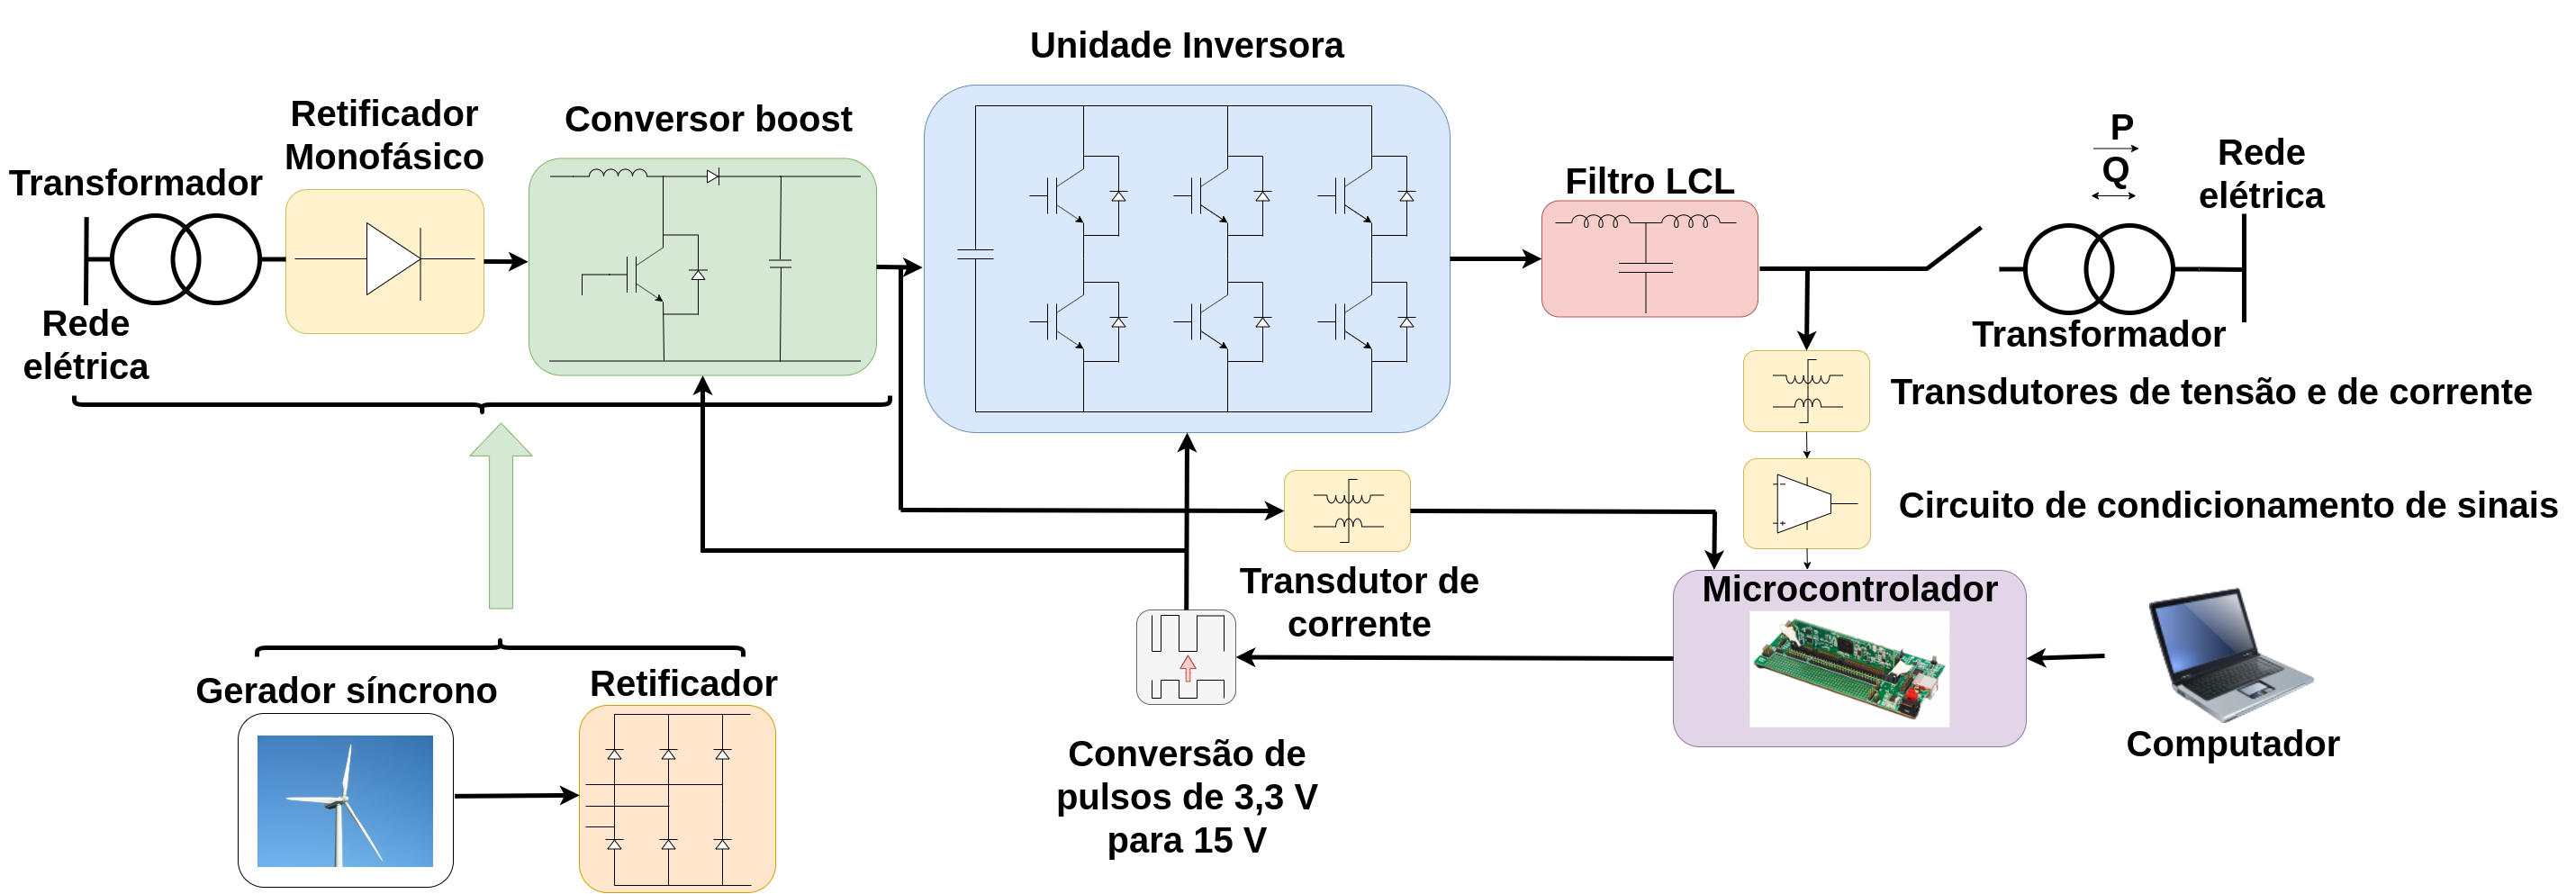
\includegraphics[scale=0.16]{figuras/Estrutura_Laboratorial.png}
    \caption{Composição da Bancada Eólica}
    \label{fig:bancada-eolica}
    \end{center}
\end{figure}

Conforme pode-se visualizar na Fig. \ref{fig:bancada-eolica}, o protótipo é constituído pelas unidades de potência e unidades de controle. 

A unidades de potência são o inversor trifásico, o filtro de acomplamento, o conversor \textit{boost}, o retificador monofásico e a própria rede elétrica. 
O conversor \textit{boost}, junto com retificador e a rede elétrica, simulam o fornecimento de potência ativa pela turbina eólica através do retificador trifásico.
A unidade de potência tem como objetivo principal a transferência de potência ativa entre o gerador síncrono, que seria a turbina éolica, e a rede elétrica.

As unidades de controle são compostas pelos transdutores de tensão e de corrente, placas de condicionamento de sinais, microcontrolador, computador e adaptadores de tensão. 
O objetivo principal das unidades de controle é o monitoramento de tensões e correntes no ponto de conexão do inversor com a rede elétrica de forma a fornecer as entradas para as iterações do algoritmo de controle.

\section{Unidades de Potência}

\subsection{Conjunto Inversor Trifásico}

A unidade de potência do inversor utilizado denomina-se SPCIT 1000-80-20. Esta, em conjunto com a unidade de controle, compõem a unidade inversora proposta, como pode ser visualizado na Fig. \ref{fig:conjunto-inversor}.
Suas principais características são:

\begin{figure}[!hbt]
	\begin{center}
    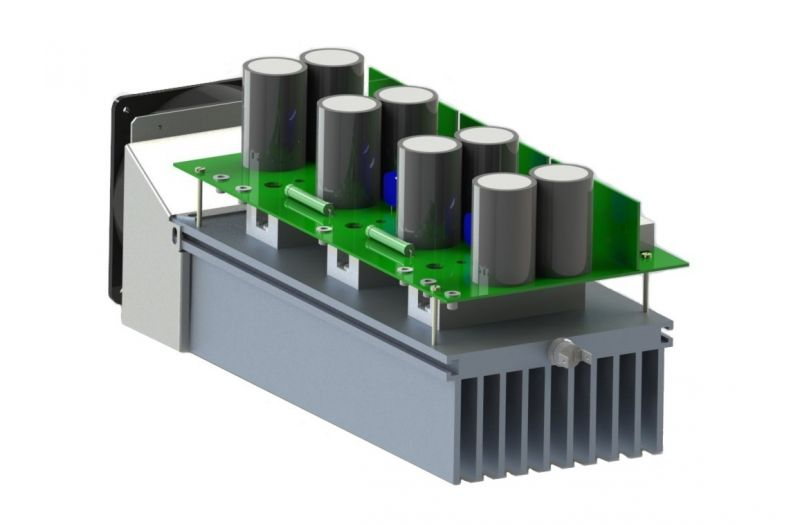
\includegraphics[scale=0.3]{figuras/conjunto_inversor_trifasico.jpg}
    \caption{Conjunto Inversor Trifásico SPCIT 1000-80-20. Fonte: Supplier}
    \label{fig:conjunto-inversor}
    \end{center}
\end{figure}

\begin{itemize}
	\item Inversor trifásico de três braços na topologia meia-ponte;
	\item Braços compostos por IGBTs do tipo LUH100G1201, conforme a Fig. \ref{fig:igbt-LUH100G1201}, equipado com \textit{gate drivers} DRO100D25A, conforme a Fig. \ref{fig:driver-DRO100D25A}.
	\item Tensão máxima de barramento: 800 $V_{CC}$ + 10 \%;
	\item Frequência máxima de chaveamento: 20 kHz;
	\item Potência Nominal: 10 kVA:
	\item Tensão de saída: 0 - 380 $V_{RMS(F-F)}$;
	\item Frequência de saída: 30 - 150 Hz;
	\item Corrente máxima de saída: 15,2 A para 380 $V_{F-F}$, tensão de barramento em 800 V, frequência de chaveamento 10 kHz;
	\item Ventilador ASA 12038DV-HB e termostato para proteção térmica.
	
\end{itemize}

\begin{figure}[!hbt]
	\begin{center}
    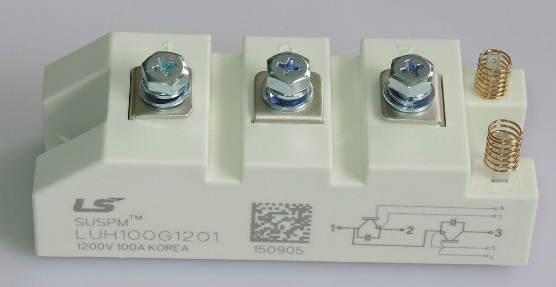
\includegraphics[scale=0.3]{figuras/LUH100G1201.png}
    \caption{IGBT LUH100G1201}
    \label{fig:igbt-LUH100G1201}
    \end{center}
\end{figure}

\begin{figure}[!hbt]
	\begin{center}
    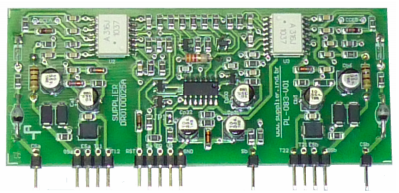
\includegraphics[scale=0.3]{figuras/driver_DRO100D25A.png}
    \caption{\textit{Gate driver} DRO100D25A. Fonte: Supplier}
    \label{fig:driver-DRO100D25A}
    \end{center}
\end{figure}

Ressalta-se que os \textit{gate drivers} possuem dois canais independentes para controle das chaves, isolação óptica, proteção contra curto-circuito através do monitoramento de $V_{ce}$, intertravamento (\textit{interlock}) com configuração de tempo morto e proteção contra subtensão na alimentação do secundário.
A tensão de acionamento dos \textit{drivers} é 15 V, sendo necessário uma interface entre a tensão de saída do microcontrolador de 3,3 V para a entrada de 15 V.

\subsection{Filtro LCL}

\subsection{Conversor \textit{Boost}}

\section{Aquisição e Condicionamento de Sinais}

A etapa de aquisição e condicionamento de sinais destina-se à correta obtenção das tensões e correntes no ponto de acomplamento do inversor com a rede elétrica, e tem como objetivo entregar os parâmetros necessários para a realização do algoritmo de controle implementado no microcontrolador.
Desta forma, é nececessário monitorar três sinais de tensão e três sinais de corrente, e também o valor de tensão no barramento CC.
Os procedimentos realizados nesta etapa são:
\begin{enumerate}
	\item Adaptação e isolação elétrica dos sinais medidos através de níveis de tensão seguros para a etapa de amostragem;
	\item Filtragem dos sinais obtidos de forma a obter os componentes em frequência desejados para o algoritmo de controle;
	\item Ajuste dos níveis de tensão dos sinais obtidos para os limites de tensão impostos pelo ADC do microcontrolador.
\end{enumerate}

O sistema de aquisição e condicionamento de sinais é constituído por:

\begin{itemize}
	\item Transdutores de tensão e corrente;
	\item Filtros \textit{anti-aliasing}, somadores e reguladores de tensão.
\end{itemize}

\subsection{Microcontrolador}

No presente trabalho optou-se pela utilização do modelo TMS320F28335 da Texas Instruments, que pode ser visualizado na Fig. \ref{fig:dsp}.
Este microcontrolador é comumente utilizado em aplicações envolvendo controle industrial de motores, inversores fotovoltaicos e eletrônica de potência \cite{texasinstruments:tms320f28335}.

\begin{figure}[!hbt]
    \begin{center}
    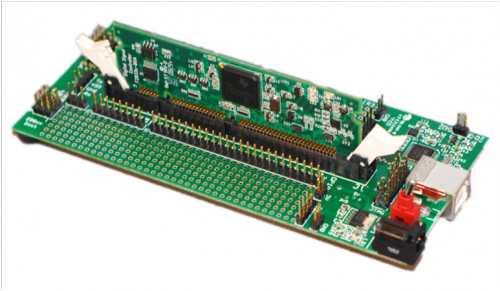
\includegraphics[scale=0.3]{figuras/tms320f28335.png}
    \caption{DSP TMS320F28335}
    \label{fig:dsp}
    \end{center}
\end{figure}

Algumas características interessantes deste microcontrolador são:
\begin{itemize}
    \item Frequência de operação: 150 MHz;
    \item Unidade de ponto flutuante (FPU) em hardware de 32 bits conforme IEEE 754;
    \item Memória RAM: 68 kB;
    \item Memória FLASH: 512 kB;
    \item ADC de 12 bits com 16 canais.
\end{itemize}

\subsection{Transdutores de Tensão e de Corrente}

Para a leitura dos sinais de tensão da rede é utilizado o transdutor de efeito Hall LV-20P mostrado na Fig. \ref{fig:transdutor_tensao}. 

\begin{figure}[!hbt]
	\centering
	\begin{subfigure}[b]{0.4\textwidth}
		\centering
		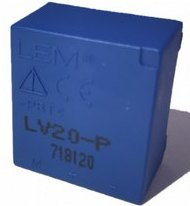
\includegraphics[width=0.5\textwidth]{figuras/Transdutor_Tensao.jpg}
		\caption{Vista frontal do trandutor}
	\end{subfigure}
	\begin{subfigure}[b]{0.4\textwidth}
		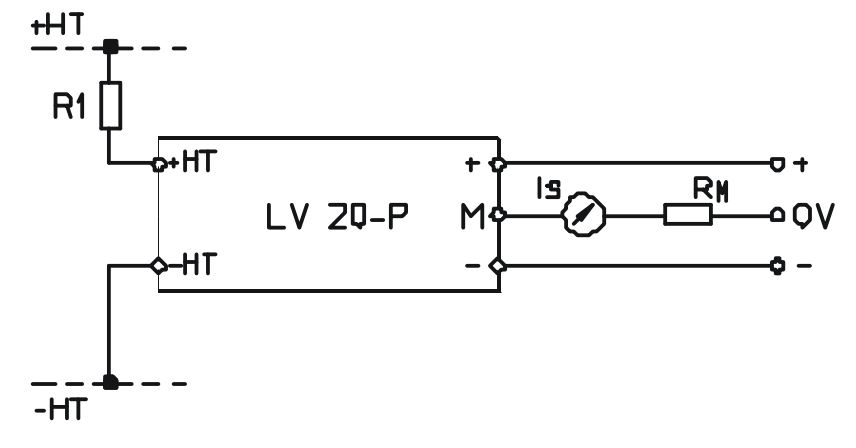
\includegraphics[width=\textwidth]{figuras/Transdutor_Tensao_Circuito.jpg}
		\caption{Circuito do transdutor}
	\end{subfigure}
	\caption{Transdutor de tensão LV-20P}\label{fig:transdutor_tensao}
\end{figure}

Já para a adaptação dos sinais de corrente é utilizado o transdutor de efeito Hall LV-55P mostrado na Fig. \ref{fig:transdutor_corrente}.

\begin{figure}
	\centering
	\begin{subfigure}[b]{0.4\textwidth}
		\centering
		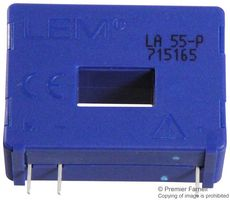
\includegraphics[width=0.5\textwidth]{figuras/Transdutor_Corrente.jpg}
		\caption{Vista frontal do trandutor}
	\end{subfigure}
	\begin{subfigure}[b]{0.4\textwidth}
		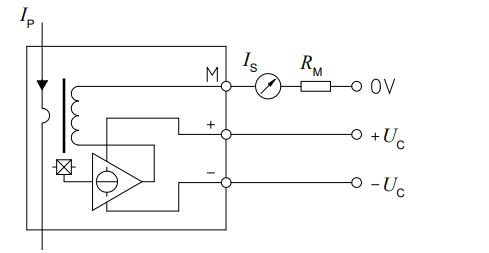
\includegraphics[width=\textwidth]{figuras/Transdutor_Corrente_Circuito.jpg}
		\caption{Circuito do transdutor}
	\end{subfigure}
	\caption{Transdutor de corrente LV-55P}\label{fig:transdutor_corrente}
\end{figure}

\subsection{Filtro \textit{Anti-Aliasing}}

	Uma vez realizada a aquisição dos sinais de interesse através dos transdutores, estes devem estar adequados para que sua manipulação por meio do microcontrolador seja possível.
	Estes sinais podem conter ruídos e transitórios eletromagnéticos inerentes à rede elétrica que são indesejáveis e tendem a provocar o denominado efeito \textit{aliasing}, que causa a sobreposição do espectro e distorções dos sinais analógicos amostrados.
	A obtenção dos sinais relevantes para este trabalho é realizada à uma frequência de amostragem $f_s$ de 10 kHz. O teorema de Nyquist define que para que o sinal analógico de interesse possa ser amostrado corretamente, a frequência $f_{max}$ deste deve ser menor ou igual à metade da frequência de amostragem, conforme a Eq. \ref{eq:freq_sinal} \cite{alanoppenheim2009}.

	\begin{align}
		f_{max} = \frac{f_s}{2}\label{eq:freq_sinal}
	\end{align}

	Com isto, utiliza-se um filtro passa-baixa do tipo \textit{Butterworth} com frequência de corte em 5 kHz e ganho K = 1. A topologia física deste é apresentada na Fig. \ref{fig:filtro-butter}.
	
\begin{figure}[!hbt]
         % Center the figure.
         \begin{center}
         % Include the eps file, scale it such that it's width equals the column width. You can also put width=8cm for example...
         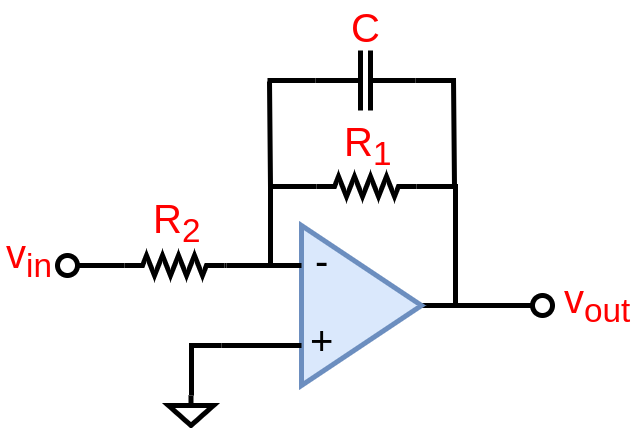
\includegraphics[scale=0.25]{figuras/Filtro_butter.png}
         % Create a subtitle for the figure.
         \caption{Topologia do filtro de Butterworth de primeira ordem utilizado na placa de condicionamento de sinais}
         % Define the label of the figure. It's good to use 'fig:title', so you know that the label belongs to a figure.
         \label{fig:filtro-butter}
         \end{center}
 \end{figure}

	A frequência de corte $f_c$ deste filtro é dado pela Eq. \ref{eq:freq_corte_butter} e o ganho $K$ é dado pela Eq. \ref{eq:ganho_butter}.
	
\begin{align}
	f_{c} = \frac{1}{2\pi R_1 C} \label{eq:freq_corte_butter} \\
	K = -\frac{R_2}{R_1}\label{eq:ganho_butter}
\end{align}

\subsection{Circuito Somador}

Um circuito com amplificador operacional na topologia de somador é necessário para que se adicione um nível DC ao sinal proviniente do filtro \textit{anti-aliasing}, de forma que o sinal a ser amostrado reproduza apenas valores positivos compatíveis com os limites de tensão do conversor A/D do microcontrolador. 
A topologia escolhida foi a de \textbf{somador não-inversor}, pois esta não altera os ângulos de fase dos sinais provenientes dos transdutores. A Figura \ref{fig:somador-ninversor} mostra o circuito do somador não inversor. A Eq. \ref{eq:circuito-somador} relaciona a tensão de saída com as tensões de entrada, onde $V_{REF}$ é a tensão de nível CC que é somada ao sinal que vem do filtro anti-aliasing, $V_1$.

\begin{align}
	V_{out} = \left(1+\frac{R_a}{R_b}\right)\left(\frac{V_1/R_1 + V_{REF}/R_2}{1/R_1 + 1/R_2}\right)\label{eq:circuito-somador}
\end{align}

\begin{figure}[!hbt]
	% Center the figure.
	\begin{center}
		% Include the eps file, scale it such that it's width equals the column width. You can also put width=8cm for example...
		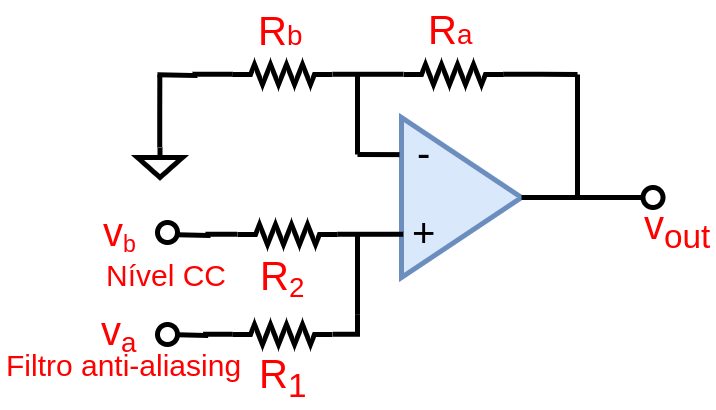
\includegraphics[scale=0.25]{figuras/Somador_Nao-Inversor.png}
		% Create a subtitle for the figure.
		\caption{Circuito somador não-inversor}
		% Define the label of the figure. It's good to use 'fig:title', so you know that the label belongs to a figure.
		\label{fig:somador-ninversor}
	\end{center}
\end{figure}

\subsection{Circuito de fornecimento de tensão CC}

Um outro circuito, anterior ao somador não-inversor, é utilizado para fornecer a tensão CC regulável ao somador.
A Fig. \ref{fig:divisor-tensao} mostra a topologia do circuito. A resistência variável conectada ao amplificador operacional permite o ajuste fino do divisor de tensão.

\begin{figure}[!hbt]
	% Center the figure.
	\begin{center}
		% Include the eps file, scale it such that it's width equals the column width. You can also put width=8cm for example...
		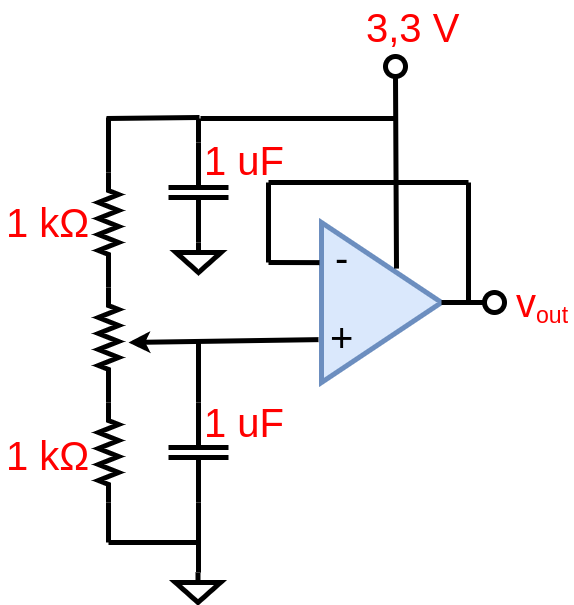
\includegraphics[scale=0.25]{figuras/divisor-tensao.png}
		% Create a subtitle for the figure.
		\caption{Divisor de tensão com resistência variável}
		% Define the label of the figure. It's good to use 'fig:title', so you know that the label belongs to a figure.
		\label{fig:divisor-tensao}
	\end{center}
\end{figure}

\subsection{Circuito Regulador de Tensão}

O circuito de regulação e filtragem de tensão destina-se ao suprimento de tensão aos amplificadores operacionais e transdutores da placa de aquisição. A Fig. \ref{fig:circuito-regulacao} mostra os componentes deste circuito. Este é basicamente composto por \textit{beads} de ferrite e capacitores destinados à minimização de ruídos existentes na tensão de suprimento da placa. A placa de aquisição de sinais é alimentada por uma fonte externa que deve dispor de tensões contínuas de +15 V e -15 V.

\begin{figure}[!hbt]
	% Center the figure.
	\begin{center}
		% Include the eps file, scale it such that it's width equals the column width. You can also put width=8cm for example...
		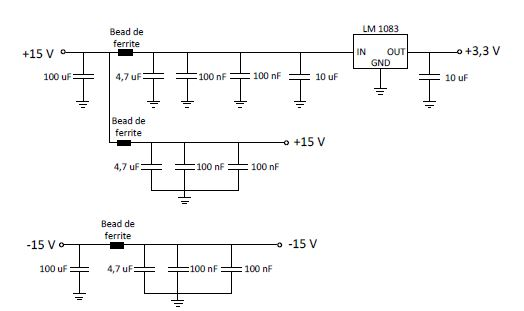
\includegraphics[scale=0.7]{figuras/circuito-regulador.JPG}
		% Create a subtitle for the figure.
		\caption{Circuito para regulação e filtragem de tensão}
		% Define the label of the figure. It's good to use 'fig:title', so you know that the label belongs to a figure.
		\label{fig:circuito-regulacao}
	\end{center}
\end{figure}